\chapter{Research methodology and implementation}
\label{ch:methodology}
In this chapter the author discusses the methodology to be followed in the experiments. This is an important step, as building it correctly will lead to significant and meaningful results.
Three phases are designed: data acquisition and preprocessing, price forecasting and predictor's importance analysis.

In the first phase, all the necessary data will be downloaded with the finest possible granularity.
When studying broader timespans, it will be aggregated.

In the last two phases the author details the analysis performed: the same procedure will be used to analyze in an hourly, daily and monthly fashion, setting specific parameters for every case.
On the other hand, for the yearly level, as there is not enough data to perform an statistical study, a descriptive and visual analysis will be performed.

During the previous years, many time series libraries have been developed for both R and Python. To choose the most adequate programming language to develop the experiments, the author will discuss the benefits and drawbacks of the two most used languages by data scientists:
\begin{itemize}
    \item \textbf{R:} An statistics-oriented programming language, having longer tradition in time series modelling. Packages as \textit{tidyverse} (great alternative to clean, manipulate and visualize data), \textit{modeltime} or \textit{fable} (time series forecasting packages) work well and are easy to use.
    \item \textbf{Python:} The currently most used Data Science language, is a general-purpose programming language. In the previous three years many new time series libraries have emerged for this language as pycaret, sktime or skforecast.
\end{itemize}

Between the two languages, the author will stick to Python. It is a general purpose language, being not only used in Data Science but in other fields as Web Development. For this project, in which APIs will be used to retrieve data, this is an advantage. Apart, the existing model explainability libraries are more advanced in Python. Finally, as the author has already worked with time series in R, it is a good opportunity to discover them in a different programming language.

The complete implementation can be found in the GitHub repository of the project \cite{project-repo}.

\subsubsection{Note on scaling and outlier detection}
In all the steps of the analysis, both when forecasting and computing SHAP values, data is scaled and outliers are detected and interpolated properly. This is because some models in use, specially those based on distances, are sensible to scale, and all the models can be affected by an unusually high or low value in the series.

When applying holdout, the scaler and outlier detector are trained only over the train partition. In the case of using cross validation, each fold is processed independently. By doing this, data leakage is prevented.

\section{Data acquisition and preprocessing}
Gathering and preparing data is a fundamental step in a Data Science project. It can take more than the half of time devoted: the data scientist needs to select the adequate variables, look for reliable sources to extract them and preprocess the data, so it's correct and accurate.

To simplify this process, the author has created two abstract classes that are implemented for each data source, as can be seen on Figure \ref{fig:data-down-prov}.

\begin{figure}[H]
\centering
    \caption{DataDownloader and DataProvider abstract classes and instance classes implementing them for each source.}
    \label{fig:data-down-prov}
    \fbox{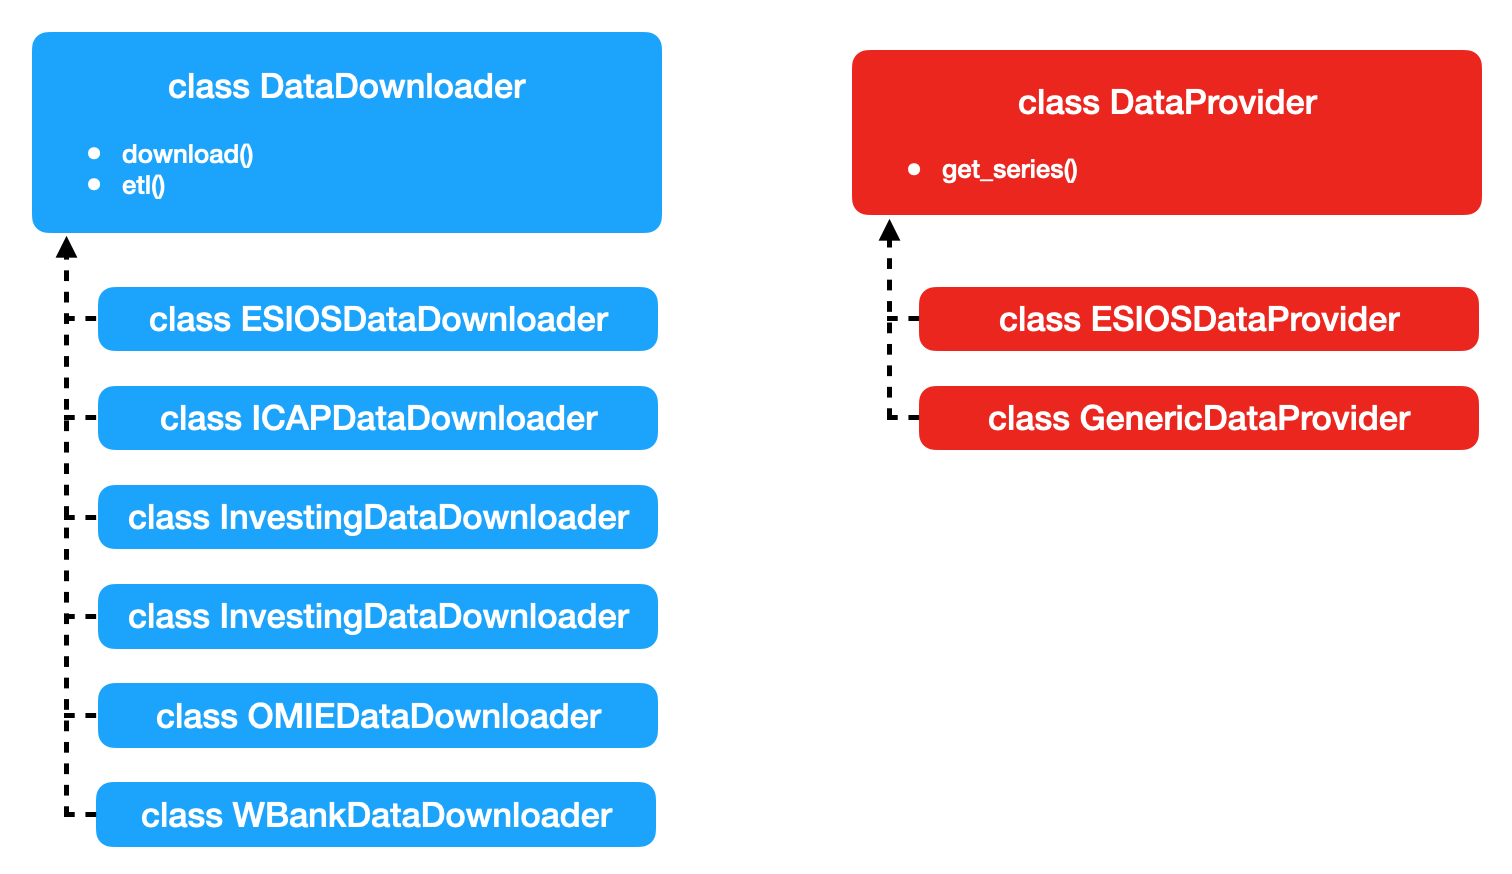
\includegraphics[scale=0.4]{images/methodology/data_down_prov}}
\end{figure}

\textit{DataDownloader} has two main methods implemented by the different materialized classes: they are \textit{downloader()} and \textit{etl()}. The first one is in charge of connecting to an API or URL and downloading the raw information on it. The second one, cleans the data and stores it in a normalized file, see Figure \ref{fig:cleandata-example}: using the same format for all data sources will simplify the manipulation process in \textit{DataProvider}. \textit{etl()} is also the place where missing values are inputted using linear interpolation or date inconsistencies due to summer/winter time changes are fixed.

For now, only ESIOS downloads the data using an API, concretely using a wrapper available at \cite{esios-api-wrapper}. For the other sources, data is downloaded manually from the browser, as most of them don't have a public API.

Each stored series has a \textit{ticker} associated. This is a name that uniquely identifies the series and can be used by \textit{DataProvider} to find it. The class has a method named \textit{get\_series()} which, given a ticker, an aggregation level (hourly, daily, monthly...) and start and end dates retrieves the information as a \textit{pandas} series. This information is retrieved from the normalized file mentioned in the previous paragraph.

A less important but also interesting class is \textit{Metadata}. It can be used by each source to store metadata in a XML file for each series, see Figure \ref{fig:metadata-example}.

\begin{figure}[H]
\centering
    \begin{subfigure}{.45\textwidth}
        \centering
        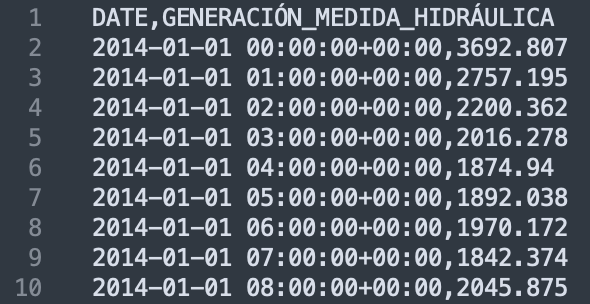
\includegraphics[width=1\linewidth]{images/methodology/clean_data_example}
        \caption{Clean data file structure after etl().}
        \label{fig:cleandata-example}
    \end{subfigure}
    \begin{subfigure}{.45\textwidth}
        \centering
        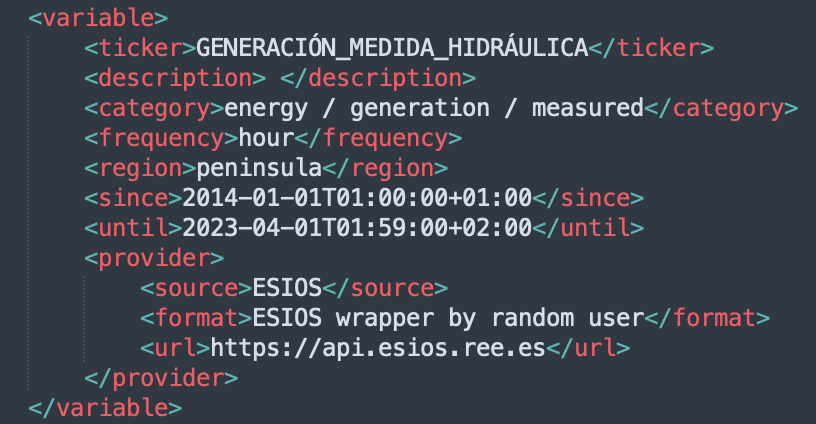
\includegraphics[width=1\linewidth]{images/methodology/metadata_example}
        \caption{Metadata file structure.}
        \label{fig:metadata-example}
    \end{subfigure}

    \caption{Example of clean data and metadata files structure, for hydropower generation.}
    \label{fig:cleandata-metadata-examples}
\end{figure}

\section{Price forecasting}
The first step of the analysis is to produce forecasts. As the author previously stated, there exist some libraries in Python that could be potential candidates to be used in this project. All of them have been extensively tested before deciding the most adequate:
\begin{itemize}
    \item \textbf{pycaret\cite{PyCaret}:} It is an AutoML library providing a time series analysis suite, apart from methods for other types of problems. It provides a very high level interface, so it's not adequate for our task.
    \item \textbf{sktime:} Probably the most advanced time series library for Python nowadays. It is compatible with \textit{scikit-learn}\cite{scikit-learn} models, contains implementations of classical models as ARIMA or ETS and lets the user build an end-to-end forecast pipeline. Nevertheless, it has a big disadvantage for us: to create the tabular form described in Figure \ref{fig:ml-arrangement} only consecutive lags can be specified. The user can't specify specific lags, something which is necessary for this project.
    \item \textbf{skforecast\cite{skforecast}:} Less advanced than the previous package, but includes the possibility of specifying specific lags. It is also compatible with \textit{scikit-learn} models.
\end{itemize}

\noindent The library finally selected to perform them is \textit{skforecast}, in combination with \textit{pandas}.

\subsubsection{Algorithms to be compared}
In Chapter \ref{ch:state-of-the-art}, different forecasting models are presented, both simple and advanced. In this project, we will focus on the use of advanced methods implemented in \textit{scikit-learn}. This is because the models on this library are directly compatible with \textit{SHAP}\cite{shap-package} package, which will be needed later to interpret predictor's importance. Statistical models libraries such as \textit{pmdarima}\cite{pmdarima} have no direct compatibility with \textbf{SHAP}, so they won't be used. Concretely, the models to be compared are the following, we will use the best performing one on each case:
\begin{itemize}
    \item k-Nearest Neighbors (kNN)
    \item Random Forests (RF)
    \item Gradient Boosted Trees (GBT)
\end{itemize}

All of them are implemented in \textit{scikit-learn} and are directly compatible with \textit{skforecast}. The first is a distance-based algorithm, while the other two are tree-based ones. Originally, other models such as Support Vector Machines were also evaluated but discarded for the final project version, as they were not producing quality results.

\subsubsection{Direct vs recursive forecasting}
Now let's talk about the strategy followed to perform forecasts. It's important to know that multi-step forecasting is being performed, as the forecast horizon will be composed of several values. There are two main strategies to perform multi-step forecasting, direct and recursive: the former creates one model for each value in the forecast horizon, the latter applies a recursive process in which each new prediction is based on the previous one \cite{direct-recursive-forecasting}, so only one model is created. See Figure \ref{fig:direct-recursive-forecasting}. Recursive strategy is what is used on this project, as it is less computationally expensive.

\begin{figure}[H]
\centering
    \begin{subfigure}{.45\textwidth}
        \centering
        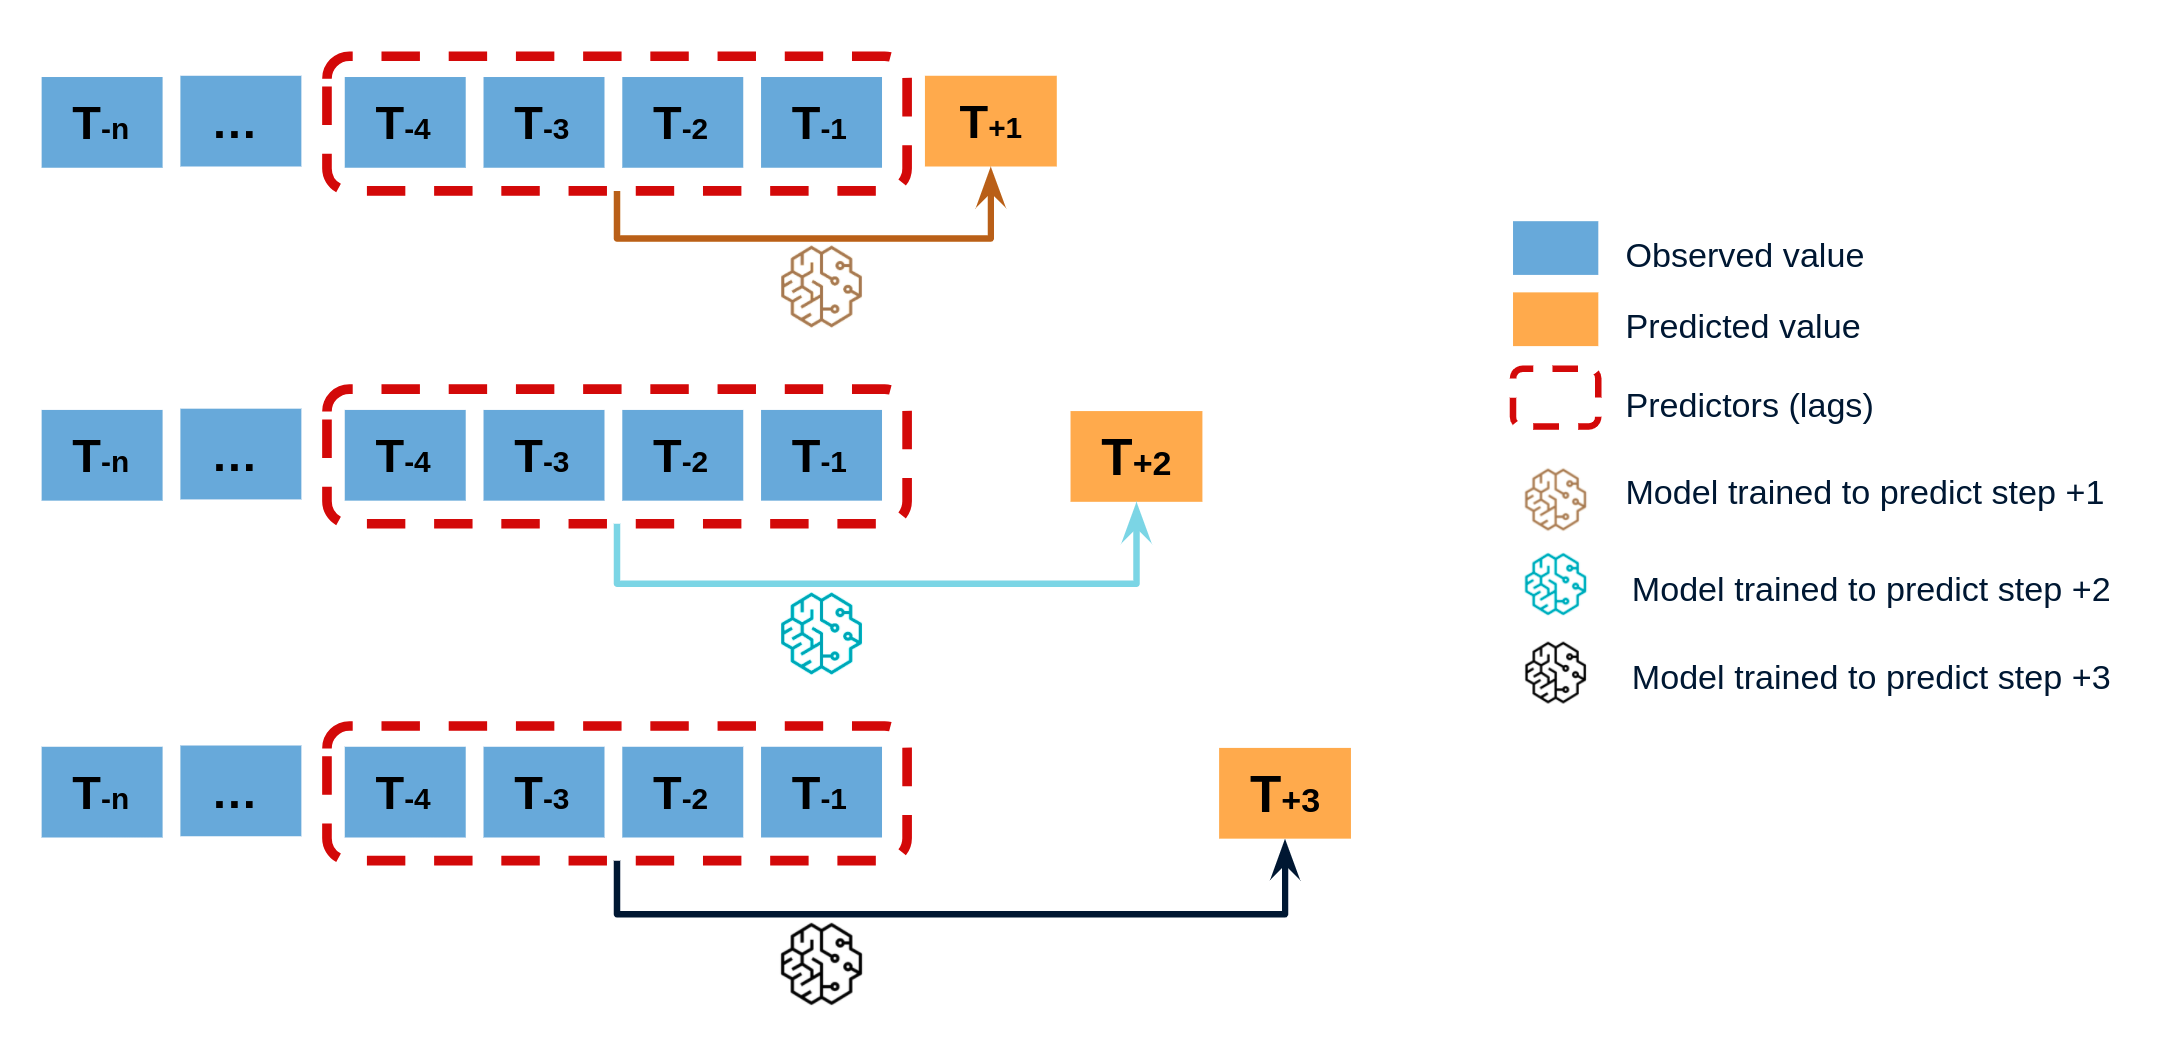
\includegraphics[width=1\linewidth]{images/methodology/direct-multi-step-forecasting}
        \caption{Direct forecasting.}
    \end{subfigure}
    \begin{subfigure}{.45\textwidth}
        \centering
        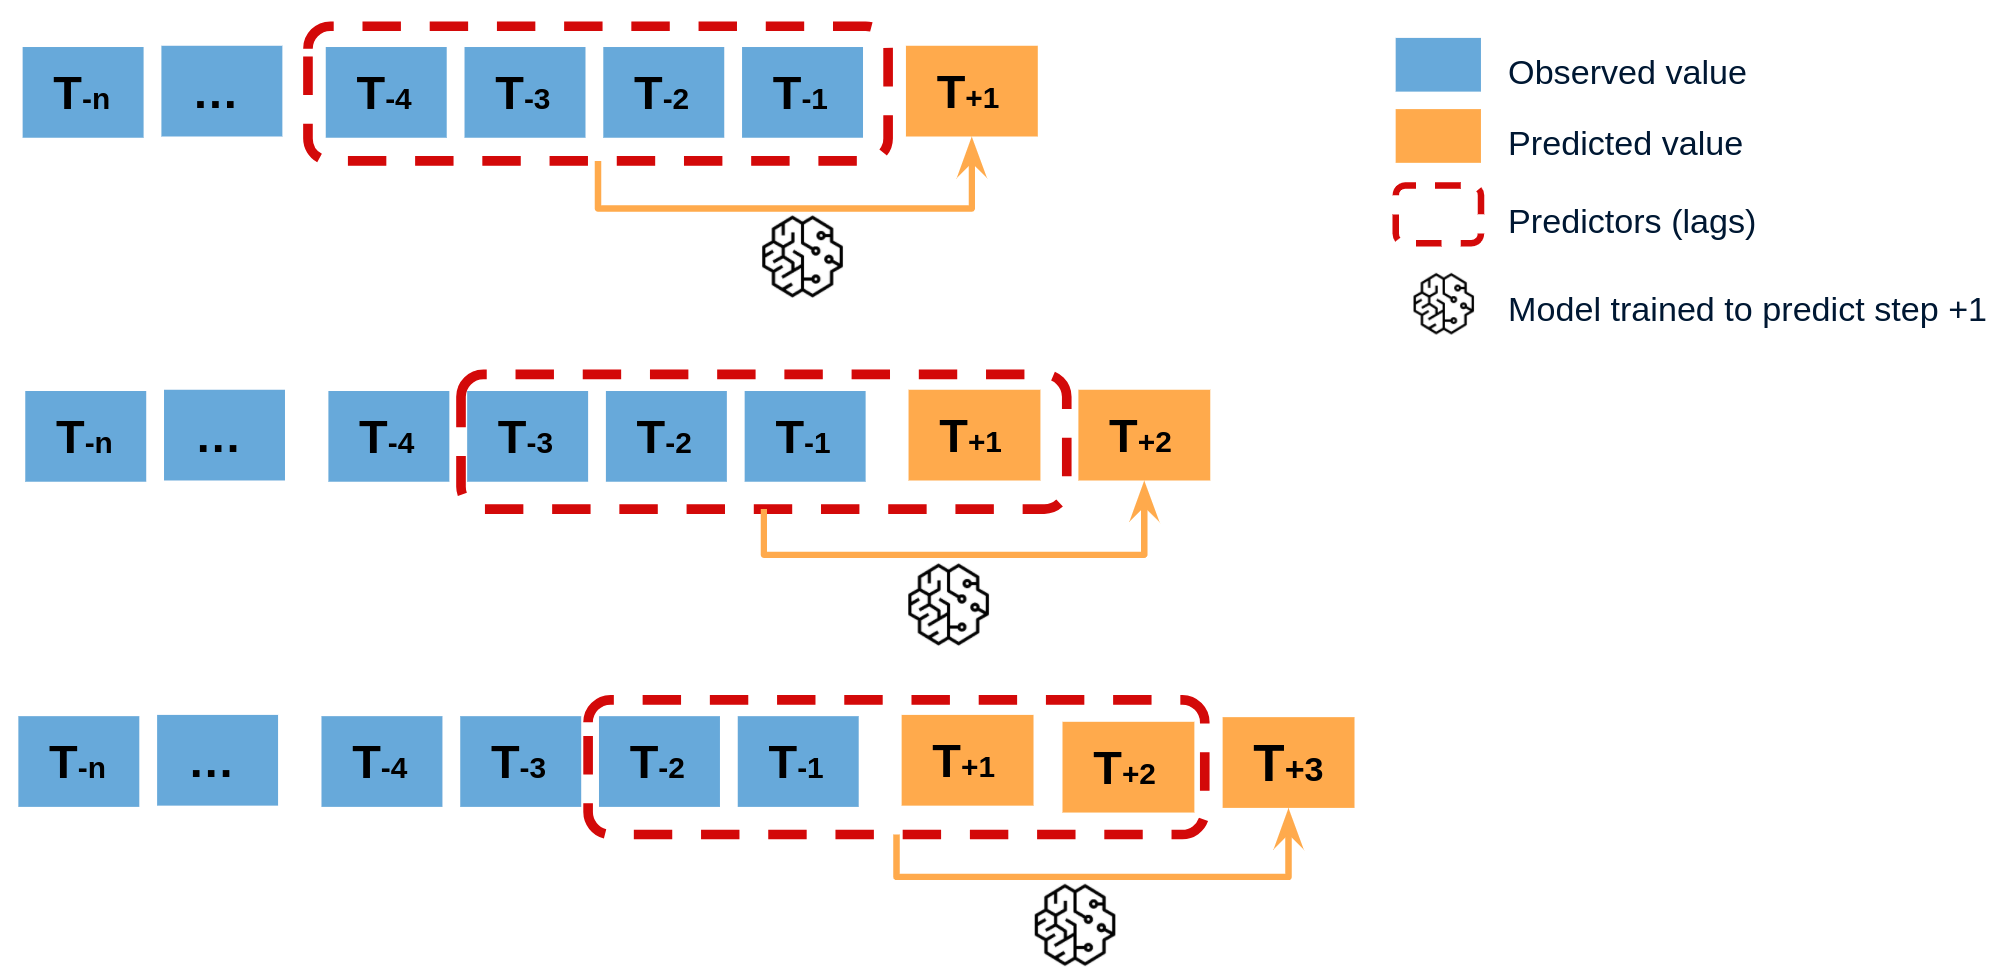
\includegraphics[width=1\linewidth]{images/methodology/recursive-mutistep-forecasting}
        \caption{Recursive forecasting.}
    \end{subfigure}

    \caption{Direct vs recursive forecasting strategies.}
    \label{fig:direct-recursive-forecasting}
\end{figure}

\subsubsection{Loss function}
To compare the performance between different models, the author has decided to use the Mean Absolute Scaled Error (MASE) function described in Equation \ref{eq:mase}. It is resistant to zero observations and scale-invariant, so if we want to compare forecasts errors of different aggregation levels is the most adequate between those presented in Chapter \ref{ch:state-of-the-art}.

\subsection{Performance evaluation}
To perform accurate forecasts, we will firstly compare the performance of the algorithms presented above using cross-validation. Once we know which one returns the highest score, we train it over all the cross-validation data and give a final estimation over a test set. See Figure \ref{fig:cross-train-test} to visualize this process.

\begin{figure}[H]
\centering
    \caption{Data splitting to peform model selection and final model performance estimation.}
    \label{fig:cross-train-test}
    \fbox{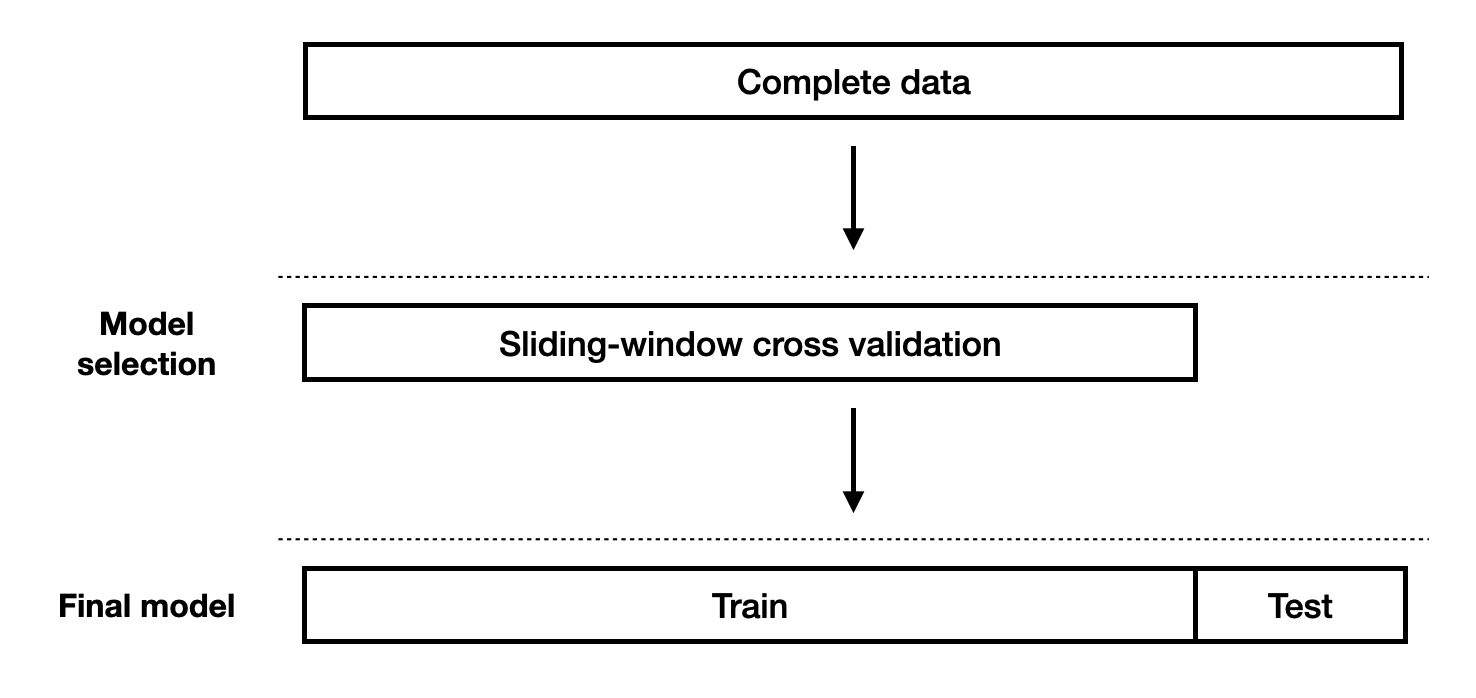
\includegraphics[scale=0.4]{images/methodology/cross_train_test}}
\end{figure}

\subsubsection{Model selection}
Two well known strategies used to divide data to perform model selection are holdout and cross-validation.
In the former, data is partitioned in two splits, train and test, e.g. 80\% train and 20\% test.
The problem with this strategy is that we are only assessing the performance of the model in a reduced portion of data.
On the other hand, if we use cross-validation we divide the data in multiple folds: on an iterative process, one is reserved for testing and the rest for training, modifying the test fold on every iteration.
At the end, we manage to assess the performance in the complete dataset.

\noindent But using k-fold cross-validation is not suitable for time series forecasting \cite{cross-validation-types}:
\begin{enumerate}
    \item Test data can appear before all the train data.
    \item Data leakage occurs if some train data appears after the test fold, as the model knows extra information about the future.
\end{enumerate}

There exist other variations that prevent these problems, for example sliding or expanding window cross-validations.
In sliding window splitters, the folds are created by scrolling a window of constant size through data.
This window is divided into train and test, maintaining the size of both partitions on all the windows.

In the case of expanding windows, its size is not constant but it grows.
Concretely, the test partition maintains the same size through different windows and the train one grows collecting all the previous observations.

In Figure \ref{fig:sliding-expanding-windows} the author shows a comparison between both strategies.

\begin{figure}[H]
\centering
    \caption{Sliding vs expanding windows \cite{sliding-expanding-windows}.}
    \label{fig:sliding-expanding-windows}
    \fbox{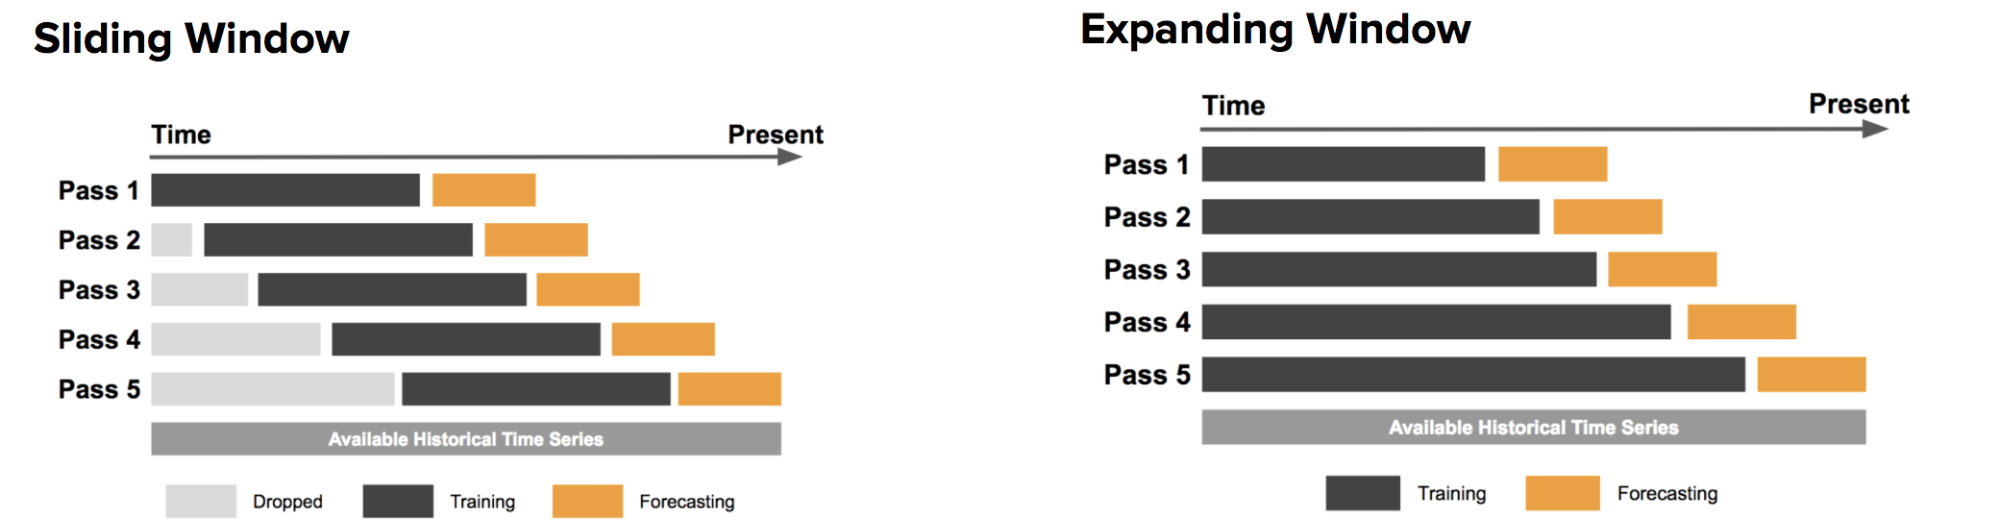
\includegraphics[scale=0.2]{images/methodology/sliding-expanding-windows}}
\end{figure}

The author believes that expanding windows are the best option for this project: data is scarce, so reusing previous observations is a possible solution to fight this problem.

Once that the data has been preprocessed and the cross-validation pipeline has been built, is time to run it.
The results will indicate which is the most suitable model.

\subsubsection{Final model}
The best model will be the one scoring the lowest MASE.

Now that the most suitable model is known, it is trained over the data used for cross validation and tested over new data that haven't been used previously, corresponding with the newest data in the series: the size of this test partition matches the size of the forecast horizon. The forecast computed over the test partition will be shown in this report, together with a final performance estimation.

\section{Predictor's importance with SHAP values}
As we studied in Chapter \ref{ch:state-of-the-art}, SHAP values are a state-of-the-art way of explaining predictor's importance in ML models. Unluckily, the existing implementation \cite{shap-package} is not directly compatible with time series libraries. On the other hand, it works with \textit{scikit-learn} models.

The strategy followed will differ from the one used in the previous section: the tabular form in Figure \ref{fig:shap-arrangement} will be built manually and scikit-learn will be directly used.

\begin{figure}[H]
\centering
    \caption{Data disposition to evaluate the influence of predictors.}
    \label{fig:shap-arrangement}
    \fbox{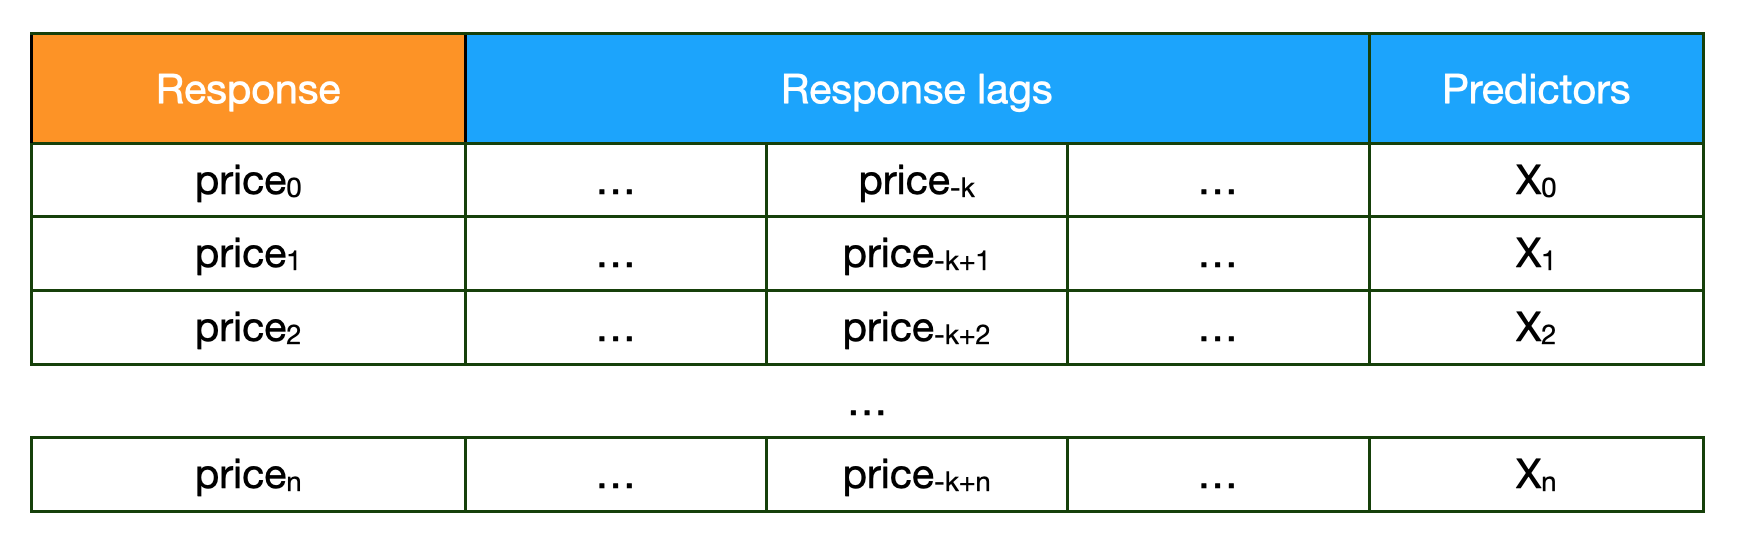
\includegraphics[scale=0.4]{images/methodology/shap_arrangement}}
\end{figure}

This table is divided in train (80\%) and test (20\%), the former is used to train the best performing \textit{scikit-learn} model and the latter is used to compute the SHAP values, see Figure \ref{fig:shap-train-test}. The model used is the one that returned the best result in forecasting.

\begin{figure}[H]
\centering
    \caption{Train/test split of the tabular data used to compute the SHAP values.}
    \label{fig:shap-train-test}
    \fbox{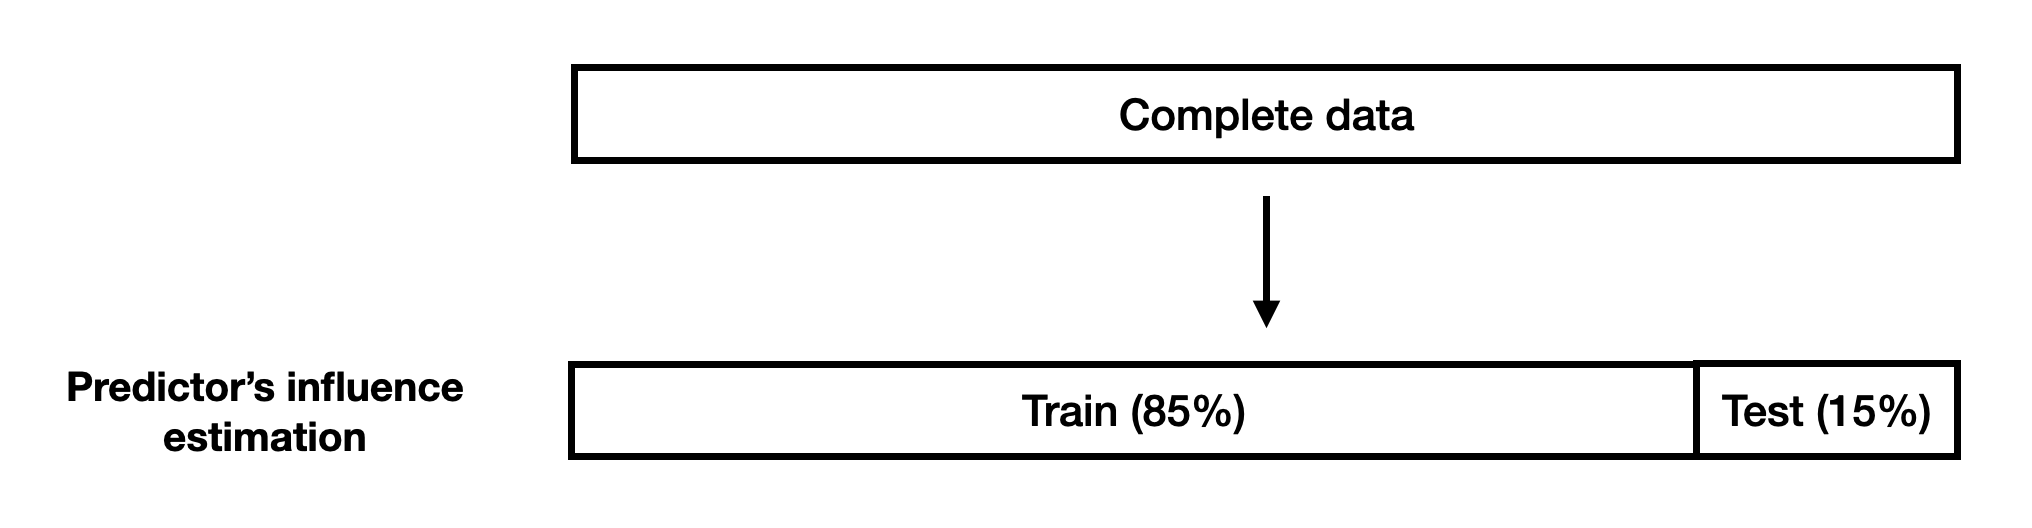
\includegraphics[scale=0.38]{images/methodology/shap_train_test}}
\end{figure}


%\begin{figure}[H]
%\centering
%    \begin{subfigure}{.95\textwidth}
%        \centering
%        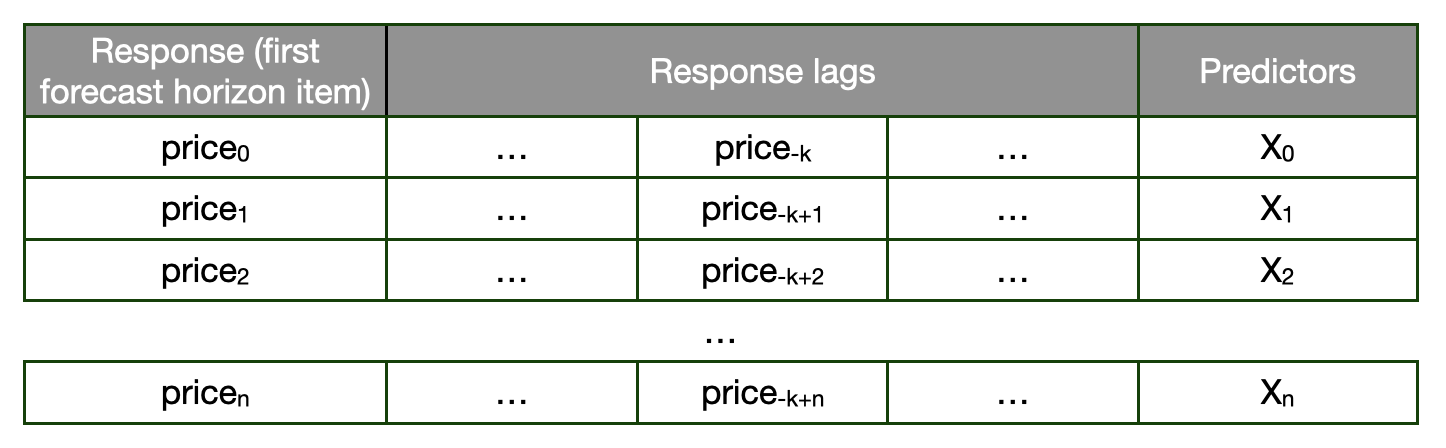
\includegraphics[width=1\linewidth]{images/methodology/shap_arrangement_first}
%        \caption{Disposition for the first value case in the forecast horizon.}
%        \label{fig:shap-arrangement-first}
%    \end{subfigure}
%    \vspace{0.3cm}
%    \begin{subfigure}{.95\textwidth}
%        \centering
%        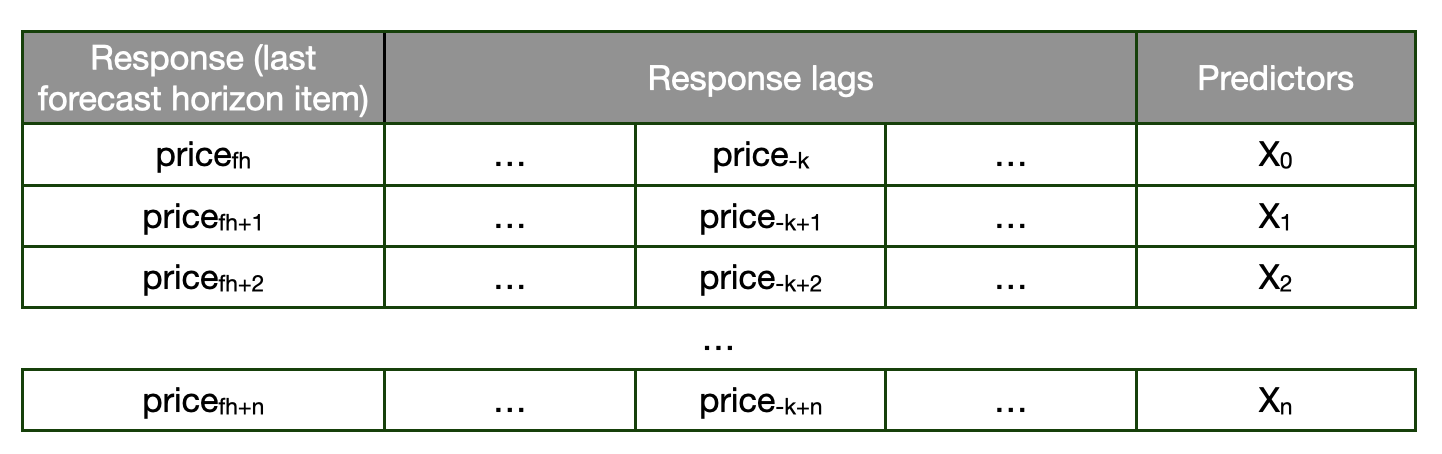
\includegraphics[width=1\linewidth]{images/methodology/shap_arrangement_last}
%        \caption{Disposition for the last value case in the forecast horizon.}
%        \label{fig:shap-arrangement-last}
%    \end{subfigure}
%
%    \caption{Data disposition to evaluate the influence of predictors.}
%    \label{fig:shap-arrangement}
%\end{figure}


%\section{Yearly forecasting}
%Judgmental forecasting